% tex file for results

% from regression_results
\par To develop linear models, we looked at the HR from the neural response 
as a single feature. Originally we used multiple regression to take into 
account the 3 different types of stimulus (pump, explode, cash-out) to see if 
the separation of these stimuli can better describe the response, but it wasn't 
that good. In figure \ref{fig:all_cond_time}, we can see the different 
conditions broken up. Using smoothed data, fourier and drift features in linear 
regression we obtained fitted values for fMRI BOLD contrast of a random 
voxel and also calculated the residuals for a random voxel for subject 001, 
voxel $(30,40,15)$ [Figure \ref{fig:fit_vs_act}, \ref{fig:fit_vs_res}].

  
\begin{figure}[ht]
\centering
\begin{minipage}[b]{0.45\linewidth}
	\centering
	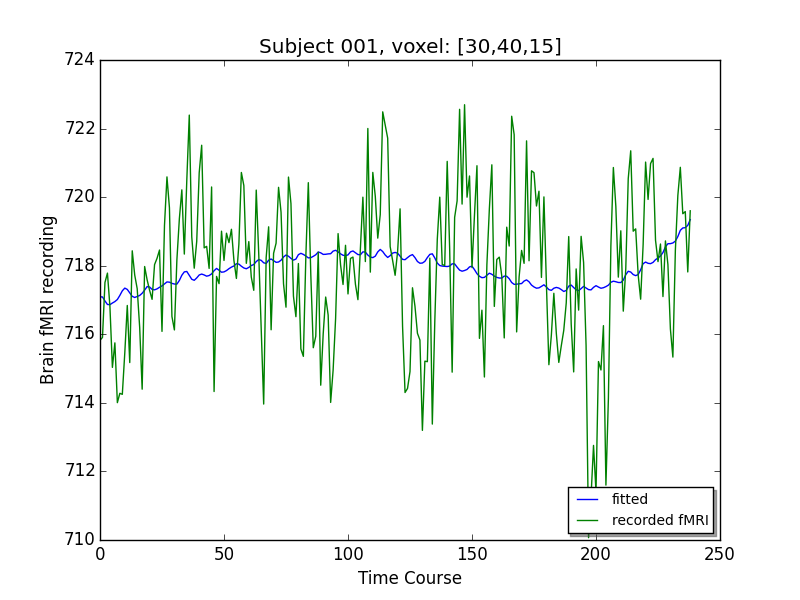
\includegraphics[width=.8\linewidth]{../images/Fitted_v_Actual.png} 
	\caption{Fitted/Predicted vs Actual fMRI BOLD contrast}
	\label{fig:fit_vs_act}
\end{minipage}	
\quad
\begin{minipage}[b]{0.45\linewidth}
	\centering
		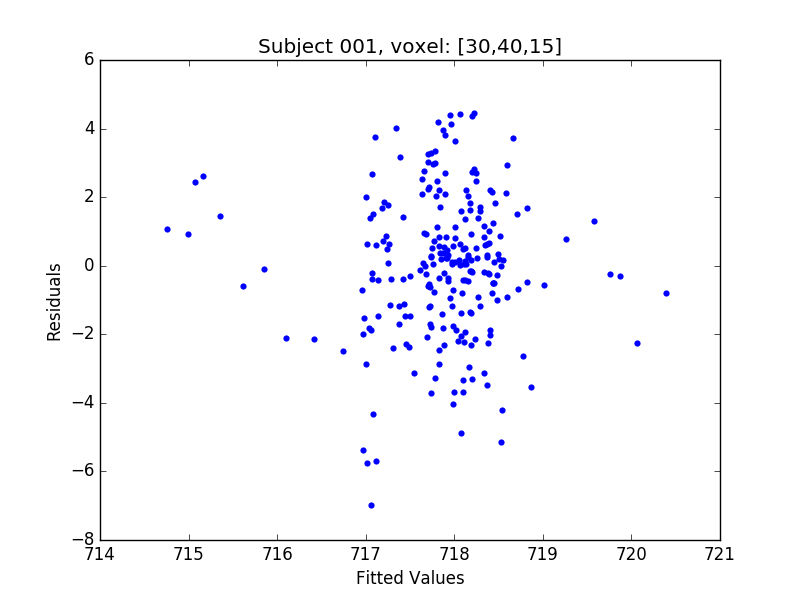
\includegraphics[width=.8\linewidth]{../images/Fitted_v_Residuals.png} 
	\caption{Fitted fMRI BOLD contrast vs Residual from Linear Regression}
	\label{fig:fit_vs_res}
\end{minipage}
\end{figure}




\begin{figure}[ht]
\centering
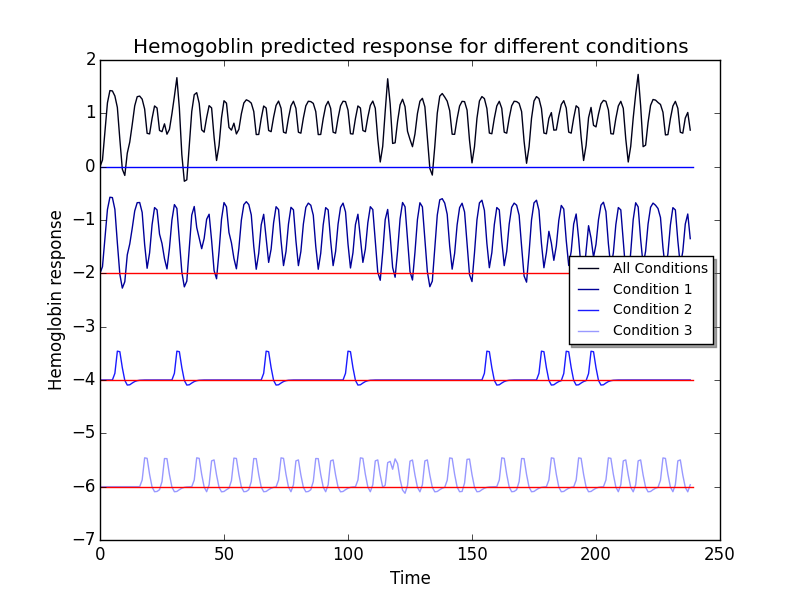
\includegraphics[scale=.5]{../images/all_cond_time}  
\caption{Plotting all predicted HR for conditions.}
\label{fig:all_cond_time}
\end{figure}

*****As we also obtained $\hat{\beta}$ values (coefficients) from the linear 
regression models, we looked at the 3-dimensional reports of the 
$\hat{\beta}$ values, a less rigorous analysis than hypothesis testing with 
t-statistics [Figure reference]. $\sim$Remove or update****



The numerous other multiple regression models discussed in 
\textit{Linear Regression} should be analyzed similarly in the future. 



% from hypothesis_results
% tex file for hypothesis testing results 
\par \indent The results of our simple linear regression t-statistic 
comparisons across subjects are shown in [Figure \ref{fig:ht}]. We can see 
each slice of the brain from top to bottom in each section of the image. The 
blue areas shows parts of the brain that had a negative t-statistic while the 
red parts of the image shows parts of the brain that had a positive t-
statistic.

\begin{figure}[ht] \centering
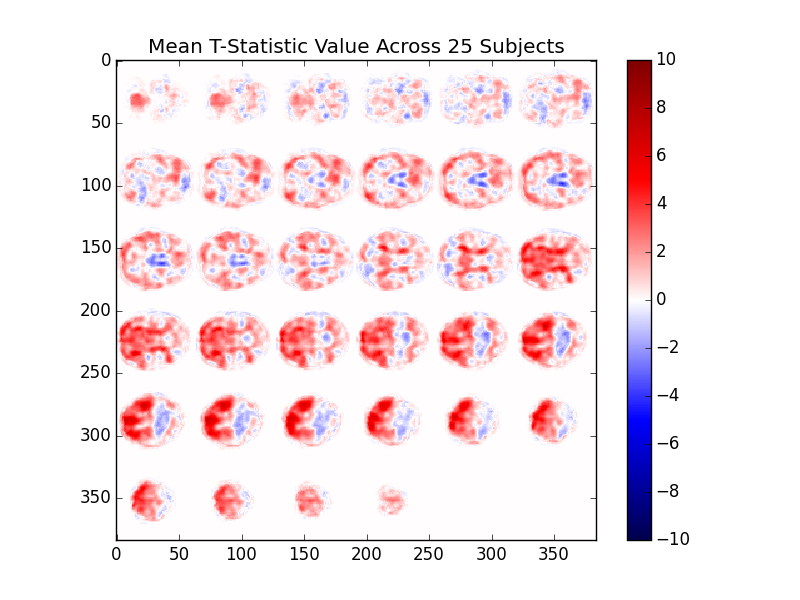
\includegraphics[scale=0.5]{../images/hypothesis_testing} \caption{Across-subject 
mean of t-Statistic per voxel.} \label{fig:ht} \end{figure}

\par The parts of the image that were cut out by the mask are white so we can 
more clearly see the contrast in our results. Based on a cursory look at this 
image, we can see a pattern of dark red (high positive t-statistics) in the lower 
left parts of the brain, and area of dark blue (high negative t-statistics) in 
the center and lower middle parts parts of the brain.


